\documentclass[11pt]{article}

\usepackage{times}
\usepackage{epsf}
\usepackage{epsfig}
\usepackage{amsmath, alltt, amssymb, xspace}
\usepackage{wrapfig}
\usepackage{fancyhdr}
\usepackage{url}
\usepackage{verbatim}
\usepackage{fancyvrb}

\usepackage{subfigure}
\usepackage{cite}
%\usepackage{cases}
%\usepackage{ltexpprt}
%\usepackage{verbatim}

%\topmargin      -0.70in  % distance to headers
%\headheight     0.2in   % height of header box
%\headsep        0.4in   % distance to top line
%\footskip       0.3in   % distance from bottom line

% Horizontal alignment
\topmargin      -0.50in  % distance to headers
\oddsidemargin  0.0in
\evensidemargin 0.0in
\textwidth      6.5in
\textheight     8.9in 


%\centerfigcaptionstrue

%\def\baselinestretch{0.95}


\newcommand\discuss[1]{\{\textbf{Discuss:} \textit{#1}\}}
%\newcommand\todo[1]{\vspace{0.1in}\{\textbf{Todo:} \textit{#1}\}\vspace{0.1in}}
\newtheorem{problem}{Problem}[section]
%\newtheorem{theorem}{Theorem}
%\newtheorem{fact}{Fact}
\newtheorem{define}{Definition}[section]
%\newtheorem{analysis}{Analysis}
\newcommand\vspacenoindent{\vspace{0.1in} \noindent}

%\newenvironment{proof}{\noindent {\bf Proof}.}{\hspace*{\fill}~\mbox{\rule[0pt]{1.3ex}{1.3ex}}}
%\newcommand\todo[1]{\vspace{0.1in}\{\textbf{Todo:} \textit{#1}\}\vspace{0.1in}}

%\newcommand\reducespace{\vspace{-0.1in}}
% reduce the space between lines
%\def\baselinestretch{0.95}

\newcommand{\fixmefn}[1]{ \footnote{\sf\ \ \fbox{FIXME} #1} }
\newcommand{\todo}[1]{
\vspace{0.1in}
\fbox{\parbox{6in}{TODO: #1}}
\vspace{0.1in}
}

\newcommand{\mybox}[1]{
\vspace{0.2in}
\noindent
\fbox{\parbox{6.5in}{#1}}
\vspace{0.1in}
}


\newcounter{question}
\setcounter{question}{1}

\newcommand{\myquestion} {{\vspace{0.1in} \noindent \bf Question \arabic{question}:} \addtocounter{question}{1} \,}

\newcommand{\myproblem} {{\noindent \bf Problem \arabic{question}:} \addtocounter{question}{1} \,}


\newcommand{\copyrightnoticeA}[1]{
\vspace{0.1in}
\fbox{\parbox{6in}{\small Copyright \copyright\ 2006 - 2014\ \ Wenliang Du, Syracuse University.\\ 
      The development of this document is partially funded by 
      the National Science Foundation's Course, Curriculum, and Laboratory 
      Improvement (CCLI) program under Award No. 0618680 and 0231122. 
      Permission is granted to copy, distribute and/or modify this document
      under the terms of the GNU Free Documentation License, Version 1.2
      or any later version published by the Free Software Foundation.
      A copy of the license can be found at http://www.gnu.org/licenses/fdl.html.}}
\vspace{0.1in}
}


\newcommand{\copyrightnotice}[1]{
\vspace{0.1in}
\fbox{\parbox{6in}{\small Copyright \copyright\ 2006 - 2014\ \ Wenliang Du, Syracuse University.\\
      The development of this document is/was funded by three grants from
      the US National Science Foundation: Awards No. 0231122 and 0618680 from
      TUES/CCLI and  Award No. 1017771 from Trustworthy Computing.
      This lab was imported into the Labtainer framework by the Naval Postgraduate 
      School, Center for Cybersecurity and Cyber Operations under National Science 
      Foundation Award No. 1438893.
      Permission is granted to copy, distribute and/or modify this document
      under the terms of the GNU Free Documentation License, Version 1.2
      or any later version published by the Free Software Foundation.
      A copy of the license can be found at http://www.gnu.org/licenses/fdl.html.}}
\vspace{0.1in}
}

\newcommand{\copyrightnoticeB}[1]{
\vspace{0.1in}
\fbox{\parbox{6in}{\small Copyright \copyright\ 2006 - 2014\ \ Wenliang Du, Syracuse University.\\
      The development of this document is/was funded by the following grants from
      the US National Science Foundation: No. 0231122, 0618680, and 1303306.
      Permission is granted to copy, distribute and/or modify this document
      under the terms of the GNU Free Documentation License, Version 1.2
      or any later version published by the Free Software Foundation.
      A copy of the license can be found at http://www.gnu.org/licenses/fdl.html.}}
\vspace{0.1in}
}


\newcommand{\nocopyrightnotice}[1]{
\vspace{0.1in}
\fbox{\parbox{6in}{\small  
      The development of this document is funded by 
      the National Science Foundation's Course, Curriculum, and Laboratory 
      Improvement (CCLI) program under Award No. 0618680 and 0231122. 
      Permission is granted to copy, distribute and/or modify this document.
      }}
\vspace{0.1in}
}

\newcommand{\idea}[1]{
\vspace{0.1in}
{\sf IDEA:\ \ \fbox{\parbox{5in}{#1}}}
\vspace{0.1in}
}

\newcommand{\questionblock}[1]{
\vspace{0.1in}
\fbox{\parbox{6in}{#1}}
\vspace{0.1in}
}


\newcommand{\minix}{{\tt Minix}\xspace}
\newcommand{\unix}{{\tt Unix}\xspace}
\newcommand{\linux}{{\tt Linux}\xspace}
\newcommand{\ubuntu}{{\tt Ubuntu}\xspace}
\newcommand{\selinux}{{\tt SELinux}\xspace}
\newcommand{\freebsd}{{\tt FreeBSD}\xspace}
\newcommand{\solaris}{{\tt Solaris}\xspace}
\newcommand{\windowsnt}{{\tt Windows NT}\xspace}
\newcommand{\setuid}{{\tt Set-UID}\xspace}
%\newcommand{\smx}{{\tt Smx}\xspace}
\newcommand{\smx}{{\tt Minix}\xspace}
\newcommand{\relay}{{\tt relay}\xspace}
\newcommand{\isys}{{\tt iSYS}\xspace}
\newcommand{\ilan}{{\tt iLAN}\xspace}
\newcommand{\iSYS}{{\tt iSYS}\xspace}
\newcommand{\iLAN}{{\tt iLAN}\xspace}
\newcommand{\iLANs}{{\tt iLAN}s\xspace}
\newcommand{\bochs}{{\tt Bochs}\xspace}

\newcommand\FF{{\mathcal{F}}}

\newcommand{\argmax}[1]{
\begin{minipage}[t]{1.25cm}\parskip-1ex\begin{center}
argmax
#1
\end{center}\end{minipage}
\;
}

\newcommand{\bm}{\boldmath}
\newcommand  {\bx}    {\mbox{\boldmath $x$}}
\newcommand  {\by}    {\mbox{\boldmath $y$}}
\newcommand  {\br}    {\mbox{\boldmath $r$}}


%\pagestyle{fancyplain}
%\lhead[\thepage]{\thesection}      % Note the different brackets!
%\rhead[\thesection]{SEED Laboratories}
%\lfoot[\fancyplain{}{}]{Syracuse University} 
%\cfoot[\fancyplain{}{}]{\thepage} 

\newcommand{\tstamp}{\today}   
%\lhead[\fancyplain{}{\thepage}]         {\fancyplain{}{\rightmark}}
%\chead[\fancyplain{}{}]                 {\fancyplain{}{}}
%\rhead[\fancyplain{}{\rightmark}]       {\fancyplain{}{\thepage}}
%\lfoot[\fancyplain{}{}]                 {\fancyplain{\tstamp}{\tstamp}}
%\cfoot[\fancyplain{\thepage}{}]         {\fancyplain{\thepage}{}}
%\rfoot[\fancyplain{\tstamp} {\tstamp}]  {\fancyplain{}{}}

\pagestyle{fancy}
%\lhead{\bfseries Computer Security Course Project}
\lhead{\bfseries SEED Labs}
\chead{}
\rhead{\small \thepage}
\lfoot{}
\cfoot{}
\rfoot{}

\usepackage{listings}
\usepackage{color}

\definecolor{dkgreen}{rgb}{0,0.6,0}
\definecolor{gray}{rgb}{0.5,0.5,0.5}
\definecolor{mauve}{rgb}{0.58,0,0.82}

\lstset{frame=tb,
  language=C,
  aboveskip=3mm,
  belowskip=3mm,
  showstringspaces=false,
  columns=flexible,
  basicstyle={\small\ttfamily},
  numbers=none,
  numberstyle=\tiny\color{gray},
  keywordstyle=\color{blue},
  commentstyle=\color{dkgreen},
  stringstyle=\color{mauve},
  breaklines=true,
  breakatwhitespace=true,
  tabsize=3
}



\begin{document}

\begin{center}
{\LARGE PLC Application Firewall and Software Whitelists}
\vspace{0.1in}\\
\end{center}


\section{Overview}
This lab explores security issues related to the use of Programmable Logic Controllers (PLCs) 
in the management of Industrial Control Systems (ICS), or similar forms of infrastructure.
You should read this ``Overview'' and the following ``Background'' section before starting the lab. 

\subsection{Learning objectives}
PLCs typically receive commands from networks containing multiple computers.  Not all of 
these networked computers are necessarily authorized to issue all commands to the PLC.
For example, some computers may be authorized to issue commands that monitor the PLC without
affecting its behavior, while other computers are designated as being able to reset or reconfigure
the PLC.  One way to enforce this type of application policy is to use a firewall that serves as
a proxy between the network computers and the PLC.  These firewalls are designed to decode the commands
destined for the PLC, and only permit those that meet the policy for which computer can issue which commands.

Limiting the computers that can alter a PLC's configuration does not ensure that the PLC will be loaded
with a valid configuration.  Malicious software on an authorized computer could load the PLC with programs
or data intended to damage the infrastructure.  One way to limit the ability of malicious software (or
individuals) to reconfigure the PLC is to enumerate a set of validated program and configuration files.
A "whitelist" of cryptographic checksums (or digests) for each valid file can then be loaded into a 
proxy that sits between the computers and the PLC.  The proxy, (or firewall), would then only permit those
files having validated digests, i.e., those whose digests appear in the whitelist.

\subsection{Simulated infrastructure control system}
This \textit{plc-app} lab simulates the system illustrated in Figure 1.  A PLC manages the water level of a creek-fed 
catfish pond, ensuring the water level stays within minimum and maximum limits.
You will interact with the sys\_management system to load a program and configuration data into the 
PLC.  You will also use the sys\_management computer to check the status of the PLC and to query which program 
and configuration data the PLC is running. 

The monitor system is used to query the status of the PLC (which can also be performed at the 
sys\_management system).  The monitor also contains the ``historian'' subsystem which keeps a running
log of the PLC status.  The monitor system must be able to continually monitor the PLC, or 
the farmer will fail the insurance company audit of his crop damage policy.

You will not have direct access to the PLC subsystem, 
though you can interact with it via the sys\_management and monitor computers.

A "Firewall" sits between the sys\_management and montior computers and the PLC.   
This device can be configured to:

\begin{enumerate}
\item Filter commands destined for the PLC, constraining the commands that may be issued from a given IP address.
\item Prevent unauthorized programs or data from being loaded into the PLC.   The firewall uses a whitelist of 
authorized MD5 digests to validate files destined for the PLC.
\end{enumerate}
The firewall is initially in its default configuration, which imposes not limits on network traffic destined
for the PLC.

\subsection {Background}
The student is expected 
to have performed the Labtainer "onewayhash" lab, or otherwise learned about 
the use of openssl to generate digests.

The student is expected to have some familiarity with the Linux command line,
the basics of the file system.

\section{Lab Environment}
This lab runs in the Labtainer framework,
available at http://my.nps.edu/web/c3o/labtainers.
That site includes links to a pre-built virtual machine
that has Labtainers installed, however Labtainers can
be run on any Linux host that supports Docker containers.

From your labtainer-student directory start the lab using:
\begin{verbatim}
    labtainer plc-app
\end{verbatim}
\noindent A link to this lab manual will be displayed.  
The resulting virtual terminals will include:
\begin{itemize}
\item A display of the status of the fish pond level, titled "Physical\_World".
\item A bash shell on the sys\_management computer.
\item A bash shell on the monitor computer.
\item A bash shell on the Firewall, titled "admin@firewall".
\item A display of the Firewall log file titled "FIREWALL\_LOG".
\end{itemize}
\noindent NOTE: When the lab starts, observe the Physical\_World window. 
The PLC is initially disabled, and thus the pump does not run and the water rises.
Throughout the lab, you will not be penalized for initial floods or other disasters.
You will, however, eventually need to configure the systems to avoid those.

\begin{figure}[H]
\begin{center}
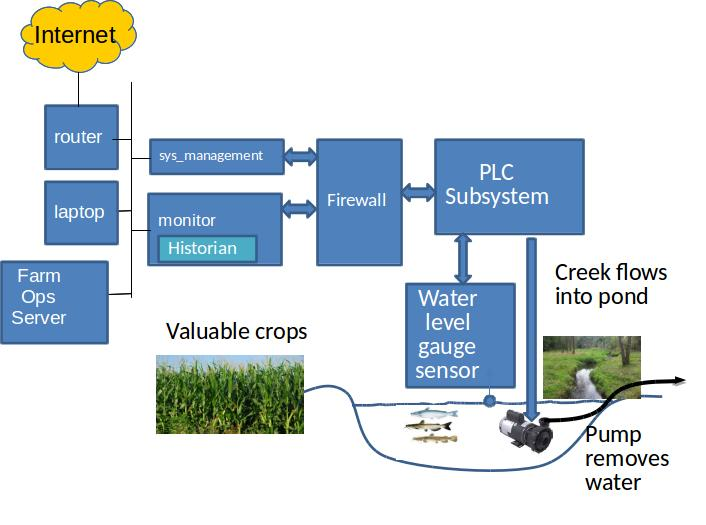
\includegraphics [width=0.8\textwidth]{plc-app.jpg}
\end{center}
\caption{Network topology for the plc-app lab}
\label{fig:topology}
\end{figure}

\section{Lab Tasks}
\subsection{Explore}
The Physical World display is notional, it is not generated by any of the components of figure 1.  It 
helps you understand what is happening in the physical world, independent of the subsystems.
Use:
\begin{verbatim}
	manage_plc status
\end{verbatim}
from the sys\_management and monitor systems to observe the state of the PLC.  Observe the log 
messages on the Firewall log.  Notice how there is periodic traffic?  That is from a service on 
the monitor computer.  If you wait long enough, you will notice that the farmer's field floods.

\subsection{Load the PLC for the rainy season}
The sys\_management computer is used by the farmer to load software into the PLC.  The
\begin{verbatim}
    manage_plc load <program> <config> 
\end{verbatim}
\noindent command is used to  load the PLC with a given program and configuration data.
It is now the rainy season, so you should specify the {\tt config\_wet.txt} configuration.  
Initialize the PLC from the sys\_management window using:
\begin{verbatim}
 manage_plc load plc config_wet.txt
\end{verbatim}
The "plc" parameter is the name of the plc program file in your home directory. This operation 
will initialize the PLC, causing to the pump to run.
The rainy season configuration file directs the PLC to keep the pond level between 15 and 25 feet,  
allowing the pond to absorb bursts of flow from the creek without flooding the fields.

Use the {\tt manage\_plc status} command to observe that the PLC is now operating, and controlling the pump.

\subsection{Constrain PLC commands based on IP address}
Go to the ``monitor'' system and use the {\tt manage\_plc status} command to view the status.
This monitor computer is in the farm yard and is used to keep an eye on the PLC.  However, a trained chicken
is known to peck the keyboard.  If you type or peck the {\tt manage\_plc reset} command from the monitor computer,
you will notice that {\tt manage\_plc status} indicates the PLC operation has stopped.

For this task, you need to configure the firewall (on the firewall computer) to allow the sys\_management computer
to issue all PLC commands, but only allow the monitor computer to issue the ``status'' and ``retrieve'' commands.
Use {\tt firewall -h} on the firewall computer to learn about configuring the firewall filters to limit PLC commands from different
IP addresses.  Use {\tt ifconfig} on the sys\_management and monitor computers to learn their addresses.  Note
that before you modify filters, you will need to stop the firewall using:
\begin{verbatim}
    sudo systemctl stop firewall
\end{verbatim}
and then, after configuring the filters, restart the firewall using:
\begin{verbatim}
    sudo systemctl start firewall
\end{verbatim}

After you have configured the firewall and restarted it, do the following:
\begin{itemize}
\item Reload the PLC from the sys\_management computer:
\begin{verbatim}
 manage_plc load plc config_wet.txt
\end{verbatim}

\item Check the status from the sys\_management computer:
\begin{verbatim}
 manage_plc status
\end{verbatim}

\item Attempt to reset the PLC from the monitor computer:
\begin{verbatim}
 manage_plc reset
\end{verbatim}

\item Confirm the PLC is still running, i.e., the reset command was blocked:
\begin{verbatim}
 manage_plc status
\end{verbatim}
\end{itemize}

Each of the above operations must yield the desired result.  If not, return to the firewall and correct its configuration.
Then repeat each and every one of the above steps to demonstrate proper application filter settings.

\subsection{Configure the PLC for the dry season}
Now that it is the dry season, Farmer Jones wants the pond to hold more water.
From the sys\_management terminal, use:
\begin{verbatim}
 manage_plc load plc config_dry.txt
\end{verbatim}
\noindent to configure the PLC for the dry season.
Then just watch what happens over the course of about a minute.
After you've watched the Physical world status window and observed a disaster, poke around a bit.

On the monitor system, view the {\tt historian.log} file in the home directory.  Do you see any
suspicious parameter settings?

From the sys\_management terminal, use:
\begin{verbatim}
 manage_plc reset
 manage_plc load plc config_dry.txt
\end{verbatim}
\noindent to reset and reload the PLC.  Watch the firewall log, do you notice any suspicious traffic?
And again review the historian.log.
Then use the {\tt manage\_plc retrieve} command to retrieve the program and configuration file 
that put the PLC into this state.  Are they the files you loaded?  Note, now is a good time
to consider revisiting the use of the {\tt openssl dgst -md5} command.

\subsection{Living with malware}
It turns out the farmer had installed a bootleg copy of pharmvilla on his laptop computer, and
that introduced malware onto the sys\_mangement computer.  That malware loads corrupt PLC programs and configuration
data.  In this lab, we assume you are unable to remove the malware or prevent it from running.  (If you
view that statement as a challenge, please complete the lab as intended before chasing the malware.)
Your task is to configure the firewall so that it only permits files having validated MD5 digests to be
loaded onto the firewall.

On the firewall computer, use the {\tt firewall -h} command to learn how to use a whitelist of MD5
digests.

Before defining a whitelist on the firewall, you must first stop it:
\begin{verbatim}
    sudo systemctl stop firewall
\end{verbatim}
and then, after configuring the whitelist, restart the firewall using:
\begin{verbatim}
    sudo systemctl start firewall
\end{verbatim}
\noindent Then use
\begin{verbatim}
 manage_plc reset
 manage_plc load plc config_dry.txt
\end{verbatim}
\noindent to restore the PLC to its desired configuration and patiently wait until the physical word
informs you that you have completed the lab -- or until you notice something not work. If something
goes wrong, review your MD5 checksums and logs and try again.

\section{Submission}
After finishing the lab, go to the terminal on your Linux system that was used to start the lab and type:
\begin{verbatim}
    stoplab 
\end{verbatim}
When you stop the lab, the system will display a path to the zipped lab results on your Linux system.  Provide that file to 
your instructor, e.g., via the Sakai site.

\copyrightnotice

\end{document}
